\documentclass{sajzk}

\usetikzlibrary {arrows.meta, angles, quotes}
\usetikzlibrary {calc}

\begin{document}
\section{Summe von Punkten an verscheiden Orten}
\label{9gpd}
\lhead{:mathe:ga:}

Sind die beinen Punte an verscheiden Stellen des Raumes zu finden, so wird ein
neuer Begriff, der Schwerpuntk eingeführt.

Seien zwei Punkte $e_1 = \mathfrak{m}_1f$ und $e_2 = \mathfrak{m}_2f$ im Raum
gegeben. Fasst man die Massen der Punkte, als Massen im Sinne der Mechanik auf
so ist de Gesammtmasse
$$\mathfrak{m} = \mathfrak{m}_1 + \mathfrak{m}_2$$
Das ist dann die Masse des gesuchten Punktes. Der Ort des Punktes ergbig sich
wie folgt:
\begin{itemize}
\item Verbinde die Beiden Punte $e_1$ und $e_2$ mit eine Linie im Raum. Der
  gesuchte Punt $s$ liegt auf dieser Linie.
\item Der genaue Ort des Punktes $s$ auf der Linie ergibt sich aus der
  Gleichgewichstlage. Wenn $r_1$ der Abstand von $s$ zu $f_1$ ist und $r_2$ der
  Abstand von $s$ zu $f_2$ ist, dann gilt
\end{itemize}
$$\mathfrak{m}_1r_1 =\mathfrak{m}_2r_2$$
oder gleichbedeutend
$$\frac{\mathfrak{m}_2}{\mathfrak{m}_1} =\frac{r_1}{r_2}$$
Somit gilt die Gleichung
$$\mathfrak{m}_1f_1 + \mathfrak{m}_2f_2 = \mathfrak{m}s$$
Hier die Konstruktion des Schwerpuntkes von zwei Punkten. Dabei haben die Massen
$\mathfrak{m}_1$ und $\mathfrak{m}_2$ das selbe Vorzeichen.

\begin{center}
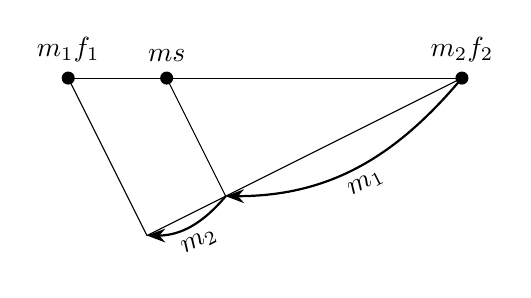
\begin{tikzpicture}[>=Stealth,
        point/.style={circle, fill=black, minimum size=1pt, scale=0.5}]
    \coordinate (f1) at (0, 0);
    \coordinate (f2) at (5, 0);
    \coordinate (h) at (1, -2);
    \coordinate (s) at ($(f1)!0.25!(f2)$);
    \coordinate (hs) at ($(h)!0.25!(f2)$);

    \draw (f1) -- (f2);
    \draw (h) -- (f2);
    \draw (h) -- (f1);
    \draw (hs) -- (s);

    \node[point, label=$\mathfrak{m}_1f_1$] at (f1) {};
    \node[point, label=$\mathfrak{m}_2f_2$] at (f2) {};
    \node[point, label=$\mathfrak{m}s$] at (s) {};

    \draw [->, thick] (f2) to [out=230, in=0]
    node [below, sloped]  (m1) {$\mathfrak{m}_1$} (hs);
    \draw [->, thick] (hs) to [out=230, in=0]
    node [below, sloped]  (m1) {$\mathfrak{m}_2$} (h);
\end{tikzpicture}
\end{center}
Wenn die Massen $\mathfrak{m}_1$ und $\mathfrak{m}_2$ unterschiedliche
Vorzeichen haben, dann sieht die Konstruktion des Schwerpuntkes so aus.

\begin{center}
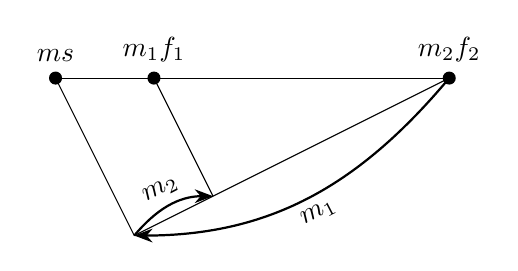
\begin{tikzpicture}[>=Stealth,
        point/.style={circle, fill=black, minimum size=1pt, scale=0.5}]
    \coordinate (s) at (0, 0);
    \coordinate (f2) at (5, 0);
    \coordinate (h) at (1, -2);
    \coordinate (f1) at ($(s)!0.25!(f2)$);
    \coordinate (hs) at ($(h)!0.25!(f2)$);

    \draw (s) -- (f2);
    \draw (h) -- (f2);
    \draw (h) -- (s);
    \draw (hs) -- (f1);

    \node[point, label=$\mathfrak{m}_1f_1$] at (f1) {};
    \node[point, label=$\mathfrak{m}_2f_2$] at (f2) {};
    \node[point, label=$\mathfrak{m}s$] at (s) {};

    \draw [->, thick] (f2) to [out=230, in=0]
    node [below, sloped]  (m1) {$\mathfrak{m}_1$} (h);
    \draw [->, thick] (h) to [out=50, in=180]
    node [above, sloped]  (m1) {$\mathfrak{m}_2$} (hs);
\end{tikzpicture}
\end{center}

\subsection{Referenzen}
\begin{itemize}
  \item \href{9wc5.pdf}{Summe von Punkten} 9wc5.tex
\end{itemize}

\subsection{Literatur}
\begin{itemize}
    \item Hermann Grassmann - Projektive Geometrie der Ebene Unter Benutzung der Punktrechnung Dargestellt Erster Band Binäres (1909) Seite 2
\end{itemize}
\end{document}
